\chapter{Objetivos y metodología}
Una vez expuestas las motivaciones y contexto del proyecto, en este capítulo se detallarán objetivos y metodología empleada. 

\label{chap:objetivos}
\section{Objetivos}
El propósito de este proyecto es la extensión y mejora de una herramienta docente para facilitar el aprendizaje de algoritmos y robótica. Para cumplir ese propósito se han fijado varios objetivos:
\begin{itemize}
    \item Añadir soporte para \textit{drone} en la plataforma, incluyendo tanto el software necesario como el modelo 3D para el entorno de \textit{A-Frame}.
    
    \item Incluir más ejercicios a \textit{WebSim}. Siendo necesario elaborar archivos de configuración para poder cambiar entre los distintos ejercicios y robots soportados. Esto incluye añadir más modelos de robots y nuevos escenarios a la plataforma.
    
    \item Añadir teleoperadores para que se puedan controlar los robots sin necesidad de programar. De esta manera se facilita la labor de los desarrolladores al poderse probar el entorno y los sensores del robot de manera sencilla.
    
    \item Incluir ejercicios competitivos de tal manera que dos usuarios puedan programar sobre el mismo escenario. Este objetivo también incluye crear un evaluador para puntuar el comportamiento de cada robot. 
    
\end{itemize}
\section{Metodología}
\label{sec:metodologia}

Para el desarrollo del proyecto se han hecho reuniones semanales con el tutor del TFG en las que se elaboraba un plan de trabajo para la semana y se revisaban las tareas concluidas. Cuando era necesario tener un desarrollo terminado, se tenía más de una reunión por semana. Este tipo de trabajo se asemeja mucho a la metodología \textit{agile}. \newline

Esta forma de trabajar consiste en estructurar el proyecto en pequeñas partes que se tienen que completar y entregar en pocas semanas. Estos plazos se llaman \textit{sprints} y en ellos el desarrollador se encarga de programar una parte especifica del proyecto. 
\section{GitHub}
\label{sec:github}
Como en la mayor parte de proyectos en la que se desarrolla \textit{software}, se ha utilizado \textit{GitHub}, que es un sistema de control de versiones que permite llevar un registro de los cambios efectuados del código del proyecto y administrarlo. Facilita trabajar en colaboración con otras personas, planificar proyectos y realizar un seguimiento el trabajo. \newline

Los archivos de cada proyecto se almacenan en repositorios, que pueden estar en local o ubicado en el almacenamiento de \textit{GitHub}. Para el desarrollo de este proyecto se han utilizado dos repositorios:  en el que se desarrolla el software principal del proyecto\footnote{\url{https://github.com/jderobot-hub/kibotics-websim}} y uno personal para llevar el registro de las tareas realizadas\footnote{\url{https://github.com/RoboticsLabURJC/2019-tfg-ruben-alvarez}}.
\newline

En el primer repositorio la metodología de trabajo ha sido creando incidencias (\textit{issues}) de algún trabajo en específico (para solucionar problemas o añadir funcionalidad) y para cerrarla se creaba una rama (\textit{branch}) realizando después un \textit{pull request} a modo parche para fusionarlo con la rama principal y así arreglar la incidencia. Se sigue esta metodología debido a que hay varios desarrolladores sobre el mismo repositorio trabajando en distintas partes de código. En la figura \ref{fig:github} se puede observar gráficamente una cronología de las ramas del repositorio durante medio mes de trabajo.

 \begin{figure}[H]
    \centering
    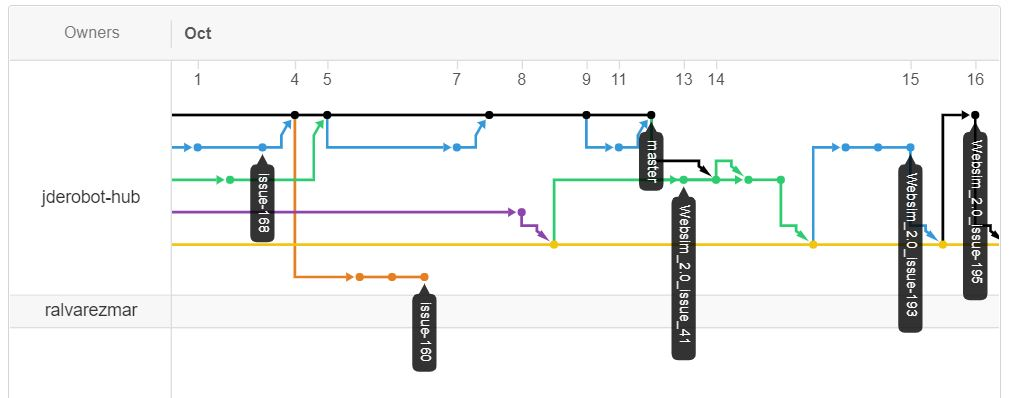
\includegraphics[width=0.8\textwidth]{img/github.jpg}
    \caption{Representación gráfica de las ramas del proyecto} \label{fig:github}
\end{figure}

En el segundo repositorio se realizó una copia del repositorio (\textit{fork}) para trabajar directamente sobre la cuenta personal de \textit{GitHub}\footnote{\url{https://github.com/ralvarezmar/2019-tfg-ruben-alvarez}}. De esta manera en primera instancia se suben los cambios al repositorio personal y, cuando hay progresos importantes, se suben todos los cambios al repositorio original. Para automatizar esta tarea se ha realizado un \textit{script} de \textit{shell} en el que el primer argumento es el mensaje del \textit{commit} y, si se escribe \textit{'-t'} después de este, se realiza la subida al repositorio copiado y al original. 

\begin{lstlisting}[language=bash, caption=\textit{Script} para subir código a \textit{GitHub}]
#!/bin/sh
if [ $# -gt 2 ]
then
	echo "usage: $1 " 1>&2
	exit 1
fi
git add .
git commit -m "$1"
git push
if [ "$2" = "-t" ]
then
	git push upstream
fi
\end{lstlisting}